


\usepackage{graphicx}   % for EPS use the graphics package instead


\begin{figure}
 
\begin{center}

   \resizebox{!}{35mm}{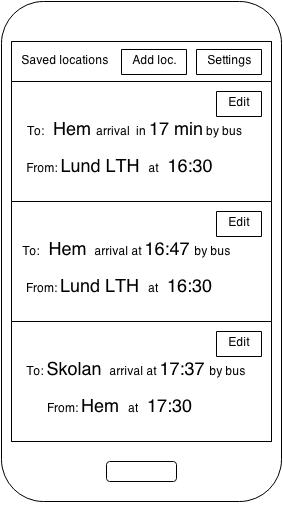
\includegraphics[width=1\textwidth]{Screens/Application.png}}
  \caption{\emph{A view of the Application main window}}
  

\end{center}    
\end{figure}

\begin{figure}
 
\begin{center}

   \resizebox{!}{35mm}{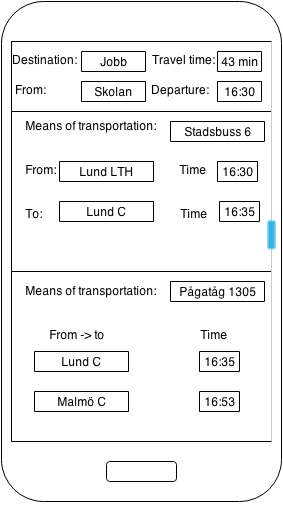
\includegraphics[width=1\textwidth]{Screens/TripInformation.png}}
  \caption{\emph{A view of the detailed information about a trip}}
  

\end{center}    
\end{figure}


\begin{figure}
 
\begin{center}

   \resizebox{!}{35mm}{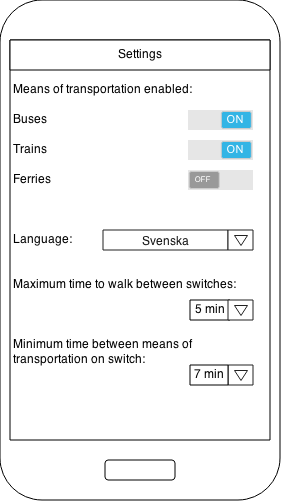
\includegraphics[width=1\textwidth]{Screens/Settings.png}}
  \caption{\emph{A view of the Settings window}}
  

\end{center}    
\end{figure}


\begin{figure}
 
\begin{center}

   \resizebox{!}{35mm}{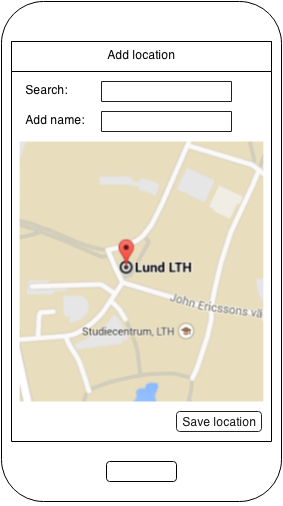
\includegraphics[width=1\textwidth]{Screens/AddDestination.png}}
  \caption{\emph{A view of the window for adding a new destination}}
  

\end{center}    
\end{figure}


\begin{figure}
 
\begin{center}

   \resizebox{!}{35mm}{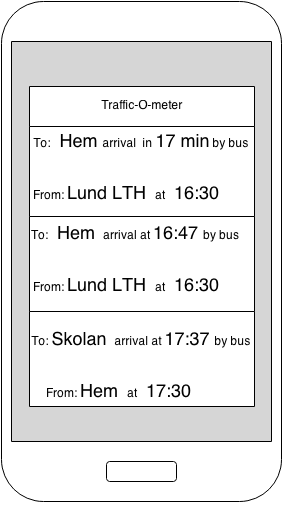
\includegraphics[width=1\textwidth]{Screens/widget.png}}
  \caption{\emph{A view of the Widget}}
  

\end{center}    
\end{figure}





